\appendix
\chapter*{Appendix}
\adjustmtc[2]

Here in the appendix can be found additional definitions (\cref{chap:additional-notions}) as well as the proofs of some of our claims that we did not put in the main corpus for the sake of clarity (\cref{chap:proofs}).

We advise the reader that is not familiar with the fields of measure theory and optimal transport to have a quick look at measure disintegration (\cref{sec:disintegration}) and at $c$-convexity (\cref{sec:cvx-analysis}) before digging into \cref{chap:stage}, where we present our contributions. More generally, if some notions are unknown to the reader, it may be worthwhile to have a look here, where they may be defined.

\Chapter{Proofs of claims}
\label{chap:proofs}


\section{Proofs of \cref{lemma:reparam,lemma:scaled-Brenier}: reparametrization of cost}
\label{subsec:proof-scaled-brenier}
        \begin{proof}[Proof of \cref{lemma:reparam}]
            Remark that the continuity of $\psi_1$ and $\psi_2$ and their inverse ensures their measurability. We have the following equalities:
            \begin{align*}
                \argmin_{\pi \in \Pi(\mu,\nu)} \int \tilde c(\psi_1 (x), \psi_2(y))\, \mathrm d\pi(x,y)& =\argmin_{\pi \in \Pi(\mu,\nu)} \int \tilde c( u,v)\, \mathrm d(\psi_1,\psi_2)\push\pi(u,v)  \\
                & =(\psi_1 ^{-1} ,\psi_2^{-1} )\push \argmin_{\tilde\pi \in \Pi(\psi_{1\pushonly} \mu, \psi_{2\pushonly}\nu)} \int \tilde c(u,v)\, \mathrm d\tilde\pi(u,v)
            \end{align*}
            since the mapping $(\psi_1 ^{-1} ,\psi_2^{-1} )\push$
            is a one-to-one correspondence from $\Pi(\psi_{1\pushonly} \mu, \psi_{2\pushonly}\nu)$ to $\Pi(\mu,\nu)$ by bijectivity of $\psi_1$ and $\psi_2$. This bijectivity ensures that any optimal deterministic transport plan $\tilde\pi\opt$ between $\psi_{1\pushonly}\mu$ and $\psi_{2\pushonly}\nu$ induces an optimal deterministic transport plan $\pi\opt$ between $\mu$ and $\nu$, and \textit{vice versa}. Writing $\tilde\pi\opt =(\id,T)\push(\psi_{1\pushonly}\mu)$, this plan $\pi\opt$ is given by
            \begin{align*}
                \pi \opt &= (\psi_1 ^{-1} ,\psi_2^{-1} )\push\tilde \pi \opt  \\
                    & =(\psi_1 ^{-1} ,\psi_2^{-1} )\push(\id,T)\push\psi_{1\pushonly} \mu \\
                    & =(\id,\psi_2^{-1}\circ T\circ\psi_1)\push\mu\,. \qedhere
            \end{align*}
        \end{proof}
        \begin{proof}[Proof of \cref{lemma:scaled-Brenier}]
            As $\psi_{1\pushonly}\mu$ has a density w.r.t.~the Lebesgue measure since $\psi_1$ is a diffeomorphism and $\psi_{1\pushonly}\mu$ and $\psi_{2\pushonly}\nu$ have compact support, Brenier's theorem states that there exists a unique optimal transport plan between $\psi_{1\pushonly}\mu$ and $\psi_{2\pushonly}\nu$ and that it is induced by a map $\nabla \phi$, where $\phi$ is a convex function. Using \cref{lemma:reparam} then gives the result.
        \end{proof}
        \begin{remark}[Discussion on the hypothesis of \cref{lemma:scaled-Brenier}]
            In the proof of \cref{lemma:scaled-Brenier}, we only needed (i) $\psi_1$, $\psi_2$ and their inverse to be measurable, (ii) $\psi_{1\pushonly}\mu$ to have a density w.r.t.~Lebesgue, and (iii) $\psi_{1\pushonly}\mu$ and $\psi_{2\pushonly}\nu$ to have compact support. Imposing $\psi_1$ to be a diffeomorphism and $\psi_2$ to be a homeomorphism ensures both (i) and (ii) and is natural to expect.
        \end{remark}

\section{Proofs of \cref{tab:twist-inner,tab:twist-quadratic}: twist conditions}
\label{sec:proof-twist-our-costs}

\noindent In this section, we prove the results summarized in the table below:
\begin{table}[H]
    \centering
    \caption{Twist conditions for the linearized GW costs (inner product and quadratic) in $\Xx=\RR^n$ and $\Yy=\RR^d$ with $n\geq d$. Given an optimal plan $\pi$, we denote by $M$ the matrix $\int y\otimes x \dd\pi(x, y)$ of size $d\times n$.}
    \label{tab:twist-our-costs}
    \begin{tabular}{llccc}
        & $\rk M$              & $=d$         & $=d-1$       & $\leq d-2$ \\\hline
        \multirow{5}*{\parbox{4.5cm}{inner product cost\\$c(x,y)=\langle M x ,\,y\rangle$}}            & twist                & $\checkmark$ & $\cdot$      & $\cdot$ \\
        & subtwist             & $\checkmark$ & $\cdot$      & $\cdot$    \\
        & 2-twist              & $\checkmark$ & $\cdot$      & $\cdot$    \\
        & $m$-twist, $m\geq 3$ & $\checkmark$ & $\cdot$      & $\cdot$    \\
        & non-degeneracy       & $\checkmark$ & $\cdot$      & $\cdot$    \\\ \\
        & $\rk M$              & $=d$         & $=d-1$       & $\leq d-2$ \\\hline
        \multirow{5}*{\parbox{4.5cm}{quadratic cost\\$c(x,y)=|x|^2|y|^2+\langle M x ,\,y\rangle$}}         & twist                & $\cdot$      & $\cdot$      & $\cdot$ \\
        & subtwist             & $\checkmark$ & $\cdot$      & $\cdot$    \\
        & 2-twist              & $\cdot$      & $\checkmark$ & $\cdot$    \\
        & $m$-twist, $m\geq 3$ & $\cdot$      & $\cdot$      & $\cdot$    \\
        & non-degeneracy       & $\sim$       & $\cdot$      & $\cdot$
    \end{tabular}
\end{table}

\begin{proof}
Let us express the gradient and Hessian of both costs $c_{\text{ip}}$ and $c_{\text{q}}$:

$$ \left\{ \begin{aligned}
	c_{\text{ip}}(x,y) & =\langle M x,\,y\rangle\\
	\nabla_{x}c_{\text{ip}}(x,y) & = M^\top y \\
	\nabla^{2}_{xy}c_{\text{ip}}(x,y) & = M^\top \\
\end{aligned}\right.\quad \text{and}\quad \left\{\begin{aligned}
	c_{\text{q}}(x,y) & =|x|^{2}|y|^{2}+4\langle Mx,\,y\rangle\\
	\nabla_{x}c_{\text{q}}(x,y) & =2|y|^{2}x+4 M^\top y\\
	\nabla^{2}_{xy}c_{\text{q}}(x,y) & =4xy^\top+4 M^\top\,.
\end{aligned}\right.$$


\paragraph{\cref{eq:twist} and \cref{eq:subtwist} conditions.} The inner product case is direct. Since $\nabla_{x}c_{\text{ip}}(x,y) = M^\top y$, $c_{\text{ip}}$ satisfies the twist condition if and only if $M$ is of full rank; in this case, the subtwist condition is also satisfied. If $M$ is not of full rank, taking any $0\neq y_1\in \ker (M^\top)$ and $y_2=0$ gives $\nabla_x c_{\text{ip}}(x,y_1)-\nabla_x c_{\text{ip}}(x,0)=0$ for all $x\in\Xx$, hence $x\mapsto c(x,y_1)-c(x,0)$ has an infinite number of critical points and the subtwist condition is not satisfied.

For the quadratic cost, we fix $y_1\neq y_2\in\Yy$. Any $x\in\Xx$ is a zero of $\nabla_x c_{\text{q}}(x,y_1)-\nabla_x c_{\text{q}}(x,y_2)$ if and only if
        \begin{equation}
            (|y_1|^2-|y_2|^2)x=-M^\top(y_1-y_2)\,.
            \label{eqn:grad2}
        \end{equation}
Let us first suppose first that $M$ is of full rank. If $|y_1|=|y_2|$, then \cref{eqn:grad2} has no solution since $y_2-y_1$ cannot be in $\ker(M^\top)$. If $|y_1|\neq|y_2|$, then \cref{eqn:grad2} has a unique solution $x\opt=-(|y_1|^2-|y_2|^2)^{-1}M^\top(y_1-y_2)$. Hence when $M$ is of full rank, the subtwist condition is satisfied but the twist condition is not. Now let's suppose that $M$ is not of full rank. We take any $0\neq z\in\ker(M^\top)$ and set $y_1=\frac12 z$ and $y_2=-\frac12 z$. Equation \cref{eqn:grad2} in $x\in\Xx$ becomes $M^\top z=0$, which is true for all $x$ and therefore has an infinite number of solutions. Hence neither the twist nor subtwist conditions are satisfied in this case.

\paragraph{\cref{eq:mtwist} condition.} Since the 1-twist condition is the twist condition, the inner product cost satisfies the $m$-twist condition for all $m\geq 2$ when $M$ is of full rank. If $M$ is not of full rank, then for any $y_0\in\Yy$, any $y\in y_0+\ker(M^\top)$ satisfies $M^\top y=M^\top y_0$, hence there is an infinite number of elements in the set $|\{y\mid \nabla_x c_{\text{q}}(x_0,y)=\nabla_x c_{\text{q}}(x_0,y_0)\}|$ for any $x_0,y_0$ and the $m$-twist condition is therefore not satisfied.

For the quadratic cost, let's consider $x_0\in\Xx$ and $y_0\in\Yy$. Let $y\in\Yy$ such that $|y|^{2}x_{0}+M^\top y=|y_{0}|^{2}x_{0}+M^\top y_{0}$. If $M$ is of full rank, then [...]\question{quid du cas de rang plein pour $m$-twist ?}. Else, denoting by $v\in\RR^d$ the right-hand side and by decomposing each vector $z\in\RR^d$ into $z=(z_M,z_\perp)\in\RR^r\times\RR^{d-r}$ where $r \defeq \rk(M)$, $$\begin{cases}
|y|^{2}x_{M}+\tilde M^\top y_{M} & =v_{M} \\
|y|^{2}x_{\perp} & =v_{\perp} \,.
\end{cases}$$
If $x_\perp$ and $v_\perp$ are not colinear then it is absurd; else, since $x_{\perp}$ and $v_{\perp}$ are fixed, this means that $|y|^{2}$ is fixed and $y$ lives on the $(d-1)$-dimensional sphere $S^{d-1}$. The first equation of the system above then gives $y_{M}=(\tilde M^\top)^{-1}(v_{M}-|y|^{2}x_{M})$; hence $y$ lives in the intersection of $S^{d-1}$ and the $(d-r)$-dimensional affine subspace of vectors $z\in\RR^d$ with fixed $z_M$, and this intersection is a $(d-r-1)$-dimensional affine sphere. Reciprocally, any $y$ in this affine sphere will satisfy $|y|^{2}x_{0}+M^\top y=v$. Hence for $m\geq2$, the $m$-twist condition is satisfied only if $d-r-1=0$, \textit{i.e.}~$\rk(M)=d-1$.


\paragraph{Non-degeneracy condition \cref{eq:non-deg}.}
The inner product case is direct, since $\det(\nabla ^{2}_{xy}c_{\text{ip}}(x,y))=\det(M)$. Regarding the quadratic cost, since $\nabla^{2}_{xy}c_{\text{q}}$ is (up to a factor and a transpose) $M+yx^\top$, \textit{i.e.}~the sum of the matrix $M$ and of a rank 1 matrix:
\begin{itemize}[nolistsep]
    \item case 1: $\rk M \leq d-2$. Then $\rk(M+yx^\top) \leq d-1$ and $\det(M+xy^\top)=0$ for all $(x,y)$.
    \item case 2: $\rk M = d-1$. Then ???
    \item case 3: $\rk M = d$. Then by the matrix determinant lemma, $\det(M+xy^\top)=(1+x^\top M^{-1}y)\det (M)$. Hence the determinant of $M+xy^\top$ is non-zero everywhere except on the set $$\left\{ (x,y)\mid x^\top M^{-1}y+1=0 \right\}\,.$$
\end{itemize}
\begin{remark}
    In dimension 1, this is indeed the parametric equation of the hyperbolae delimiting the submodularity region. \qedhere
\end{remark}
\end{proof}



\section{Proof of \cref{prop:selection-manifold}: measurable selection of maps on manifolds}
\label{sec:appendix-proof-fontbona-manifold}
The proof is essentially an adaptation of the one of \cite{fontbona2010measurability}, with additional care required due to the fact that we do not have access to a linear structure on the manifold $M$. It relies on measurability of set-valued maps (see \cite[Ch.~5 and 14]{rockafellar2009variational} and \cref{sec:measurable_set_valued} for a summary).

The crucial point regarding measurability is the following proposition.

\begin{proposition}\label{prop:Bnk_measurable}
    The set
    \begin{equation}
        B_{n,k} = \{ (u,x),\ T_u(x) \in A_{n,k} \}.
    \end{equation}
    is measurable.
\end{proposition}

\noindent Its proof relies on a core lemma:

\begin{lemma}\label{lemma:ferme_mesurable}
    Let $F \subset M$ be a closed set. Then the set
    \[ B_F = \{ (u,x),\ T_u(x) \in F \} \]
    is measurable.
\end{lemma}

\noindent The key will be to identify this set as the domain of a measurable set-valued map, see \cref{sec:measurable_set_valued}.

\begin{proof}[Proof of \cref{lemma:ferme_mesurable}]
Observe that $B_F = \{(u,x),\ (\{x\} \times F) \cap \graph(T_u) \neq \varnothing\}$, where $\graph(T_u) = \{(x,T_u(x)),\ x \in M\}$ denotes the topological closure of the graph of the optimal transport map $T_u$ that pushes $\mu_u$ onto $\nu_u$.
Let $S_1 : (u,x) \mapsto \{x\} \times F$ and $S_2 : (u,x) \mapsto \graph(T_u)$, so that $B_F = \mathrm{dom}(S)$, where $S(x) = S_1(x) \cap S_2(x)$. According to \cref{prop:intersection_of_measurable}, given that $S_1$ and $S_2$ are closed-valued, if they are measurable, so is $S$, and so is $B_F$ as the domain of a measurable map. The measurability of these two maps can be easily adapted from the work of \cite{fontbona2010measurability}, we give details for the sake of completeness.

\textbf{Measurability of $S_1$:} Let $O \subset M \times M$ be open. For any $z \in F$, if $x,z \in S_1^{-1}(O) = \{x,\ \{x\} \times F \cap O \neq \varnothing \}$, we have $\epsilon > 0$ such that $B(x,\epsilon) \times \{z\} \subset O$ (since $O$ is open), and thus $B(x,\epsilon) \times F \cap O \neq \varnothing$, proving that there is a neighborhood of $x$ included in $S_1^{-1}(O)$ which is thus open (thus measurable), hence the measurability of $S_1$.

\textbf{Measurability of $S_2$:} Given that $u \mapsto (\mu_u,\nu_u)$ is measurable by assumption, and that measurability is preserved by composition, we want to show that (i) the map $S : (\mu,\nu) \mapsto \Pi(\mu,\nu)$ (the set of optimal transport plans between $\mu$ and $\nu$ for the quadratic cost on $M$) is measurable and (ii) the map $U : \pi \in P(M)^2 \mapsto \supp\pi$ satisfies $U^{-1}(O)$ is open for any open set $O \subset P(M^2)$. From these two points, we get that $(U \circ S)^{-1}(O)$ is measurable, thus the measurability of $S_2$.

To get (i), observe first that $S$ is closed-valued, so that it is sufficient to prove that $S^{-1}(C)$ is measurable for any closed set $C \subset P(M)^2$ according to \cref{prop:equiv_measure_closedvalued}. Let $C \subset P(M^2)$ be closed. Then, $S^{-1}(C) = \{(\mu,\nu),\ \Pi\opt(\mu,\nu) \cap C \neq \varnothing \}$, and consider a sequence $(\mu_n, \nu_n)_n$ in $S^{-1}(C)$ that converges to $(\mu,\nu)$ for the weak topology. Let $\pi_n \in \Pi\opt(\mu_n,\nu_n) \cap C$. According to \cite[Thm.~5.20]{villani2009optimal}, $(\pi_n)_n$ admits a weak limit $\pi$ in $\Pi\opt(\mu,\nu)$, but also since $C$ is closed, $\pi \in C$, so that $(\mu,\nu) \in S^{-1}(C)$ that is closed (hence measurable), proving the measurability of $S$.

(ii) simply follows from the fact that $U^{-1}(O) = \{ \pi,\ \supp\pi \cap O \neq \varnothing \} = \{ \pi,\ \pi(O) > 0 \}$ that is open. Indeed, the Portmanteau theorem gives that if $\pi_n \to \pi$ (weakly) and $\pi_n(O) = 0$, then $0 = \liminf \pi_n(O) \geq \pi(O) \geq 0$, so $\pi(O) = 0$. The complementary set of $U^{-1}(O)$ is closed, that is $U^{-1}(O)$ is open.
\end{proof}

\begin{proof}[Proof of \cref{prop:Bnk_measurable}]
This follows from the fact that $A_{n,k}$ can be inner-approximated by a sequence of closed set $F_j \subset A_{n,k}$ and the fact that the $B_{F_j}$ are measurable.
\end{proof}

We can now prove our main theorem. The proof is clearly inspired from the one of \cite{fontbona2010measurability}, though it requires, in few places, careful adaptation.

\begin{proof}[Proof of \cref{prop:selection-manifold}]
Recall that we assume that $M = \bigsqcup_n A_{n,k}$. For each $n,k$, select (in a measurable way) a $a_{n,k}$ in $A_{n,k}$. Then, define the map
\begin{equation}
    T^{(k)} : (u,x) \mapsto a_{n,k},\ \text{ such that } T_u(x) \in A_{n,k}.
\end{equation}
This map is measurable. Indeed, the map $\Phi_k : (u,x) \mapsto A_{n,k}$ where $T_u(x) \in A_{n,k}$ is measurable, because $\Phi_k^{-1}(O) = \bigcup_n B_{n,k} \cap O$ that is measurable.

Now, for two maps $f,g : B \times M \to M$, let $D_1$ denotes the natural $L_1$ distance on $M$, that is
\begin{equation}
    D_1(f,g) = \int_B \int_M d(f(u,x), g(u,x)) \dd \mu_u(x)  \dd m(u)\,.
\end{equation}
This yields a complete metric space, and we can observe that $(T^{(k)})_k$ is a Cauchy sequence for this distance. Indeed, for $k \leq j$ two integers, recall that we assume that $(A_{n,j})_n$ is a refinement of $(A_{n,k})_n$, yielding
\begin{align*}
    D_1(T^{(k)}, T^{(j)}) &= \int_{B} \int_M d(T^{(k)}(u,x), T^{(j)}(u,x)) \dd \mu_u (x) \dd m(u) \\
    &= \int_{B} \int_M \sum_n \sum_{n' : A_{n',j} \subset  A_{n,k}}  1_{B_{n',j}}(u,x) \cdot d(a_{n,k}, a_{n',j}) \dd \mu_u(x) \dd m(u) \\
    &= \int_B \int_M \sum_n \sum_{n' : A_{n',j} \subset  A_{n,k}} d(a_{n,k},a_{n',j}) \dd \nu_u(A_{n',j}) \dd m(u) \\
    &\leq 2^{-k}
\end{align*}
where we use that for all $u$, $\int_{x \in M} 1_{B_{n',j}}(u,x) \dd \mu_u(x) = \nu_u(A_{n',j})$ by construction (recall that $(u,x) \in B_{n',j} \Leftrightarrow T_u(x) \in A_{n',j} \Leftrightarrow x \in \mu_u(T_u^{-1}(A_{n',j})) = T_u \# \mu_u(A_{n',j})$ and $T_u$  transports $\mu_u$ onto $\nu_u$), and then that the diameter of the partition $A_{n,k}$ is less than or equal to $2^{-k}$ and that $\nu_u$ and $m$ are probability measures.

Now, let $T$ denote the limit of $(T^{(k)})_k$ (that is measurable). It remains to show that $T(u,x) = T_u(x)$, $m$-a.e. This can be obtained by proving that
\begin{equation}
    \int g(x) f(T(x,u)) \dd \mu_u(x) = \int g(x) f(T_u(x)) \dd \mu_u(x),
\end{equation}
for any pair $f,g : M \to \RR$ of bounded Lipschitz-continuous functions \cite[Lemma 2.24]{van2000asymptotic}.

As in \cite{fontbona2010measurability}, let $ \|f\| = \sup_{x \neq y} \frac{|f(x) - f(y)|}{d(x,y)} + \sup_x |f(x)|$. The difference between these two terms can be bounded using the partition $(A_{n,k})_n$. We have for $m$-a.e.~$u$:

\begin{align}
    &\left| \int g(x) f(T_u(x)) \dd \mu_u(x) - \int g(x) f(T(u,x)) \dd \mu_u(x) \right| \\
    \leq &\left| \int g(x) f(T_u(x)) \dd \mu_u(x) - \int g(x) f(T^{(k)}(u,x)) \dd \mu_u(x) \right| + \|g\| \|f\| \int d\left( T^{(k)}(u,x), T(u,x) \right) \dd \mu_u(x).
\end{align}
Since $T^{(k)} \to T$ in $D_1$, it implies that up to a subsequence, $\int_x d(T^{(k)}(u,x), T(u,x)) \dd \mu_u(x) \to 0$ as $k \to \infty$ for $m$-a.e.~$u$.

To treat the first term and show that it goes to $0$ as $k \to \infty$ for a subset of $B$ with full $m$-measure, we write for $m$-a.e.~$u$:
\begin{align*}
    &\left| \int g(x) f(T_u(x)) \dd \mu_u(x) - \int g(x) f(T^{(k)}(u,x)) \dd \mu_u(x) \right| \\
    \leq &\int |g(x)| \left| f(T_u(x)) - f(T^{(k)}(u,x))\right| \dd \mu_u(x) \\
    \leq &\|g\| \|f\| \int d(T_u(x),T^{(k)}(u,x)) \dd \mu_u(x) \\
    \leq &\|g\| \|f\| 2^{-k} \sum_n \nu_u(A_{n,k})\to 0\,.
\end{align*}
This concludes the proof.
\end{proof}





\Chapter{Additional notions}
\label{chap:additional-notions}

In this chapter, we report some mathematical definitions and results that will be useful for our study. The most important ones are those on measure theory (\cref{sec:meas-th}) that we need for constructing optimal maps in \Cref{chap:stage}---especially the disintegration theorem (\cref{sec:disintegration})---, and the definition of $c$-convexity (\cref{sec:cvx-analysis}), crucial in optimal transport theory.

\section{Notions of measure theory}
    \label{sec:meas-th}
    \subsection{Basics}
        \begin{defi}[Atom]\label{def:atom}
            An \emph{atom} is a set of positive measure which contains no nontrivial smaller measurable sets. A measure $\mu\in\Pp(\Xx)$ is therefore said to be \emph{atomless} if for any Borel set $A$ with $\mu(A)>0$ there exists a measurable subset $B$ of $A$ such that $\mu (A)>\mu (B)>0$.
        \end{defi}
        \begin{example}
            In $\RR^d$, an atomless measure is a measure that does not put mass on any point.
        \end{example}
        \begin{defi}[Support]\label{def:support}The \emph{support} $\supp\mu\subset \Xx$ of a measure $\mu\in\Pp(\Xx)$ is the smallest closed set $C$ such that $\Xx\setminus C$ has $\mu$-measure zero.\end{defi}
        \begin{defi}[Absolute continuity]\label{def:ac}
            A measure $\mu\in\Pp(\Xx)$ is \emph{absolutely continuous with respect to a measure} $\lambda$ (often the Lebesgue, Hausdorff or volume measures), written $\mu\ll\lambda$, if for every $\lambda$-measurable set $A$, $\lambda(A) = 0$ implies $\mu (A)=0$.
        \end{defi}
        \begin{theorem}[Radon--Nikodym theorem]
            In the same setting where $\mu \ll \lambda$, there exists a measurable function $\rho:X\to [0,\infty )$ such that for any measurable set $A\subset \Xx$,
            $$\mu (A)=\int _{A}\rho\,\mathrm d\lambda\, .$$
            The function $\rho$ satisfying the above equality is uniquely defined up to a $\lambda$-null set. $\rho$ is commonly written $\frac {\mathrm d\nu }{\mathrm d\mu }$ and is called the \emph{Radon--Nikodym derivative}. We say that $\mu$ has a \emph{density} $\rho$ with respect to $\lambda$.
        \end{theorem}
        \begin{defi}[Metric measure space \cite{memoli2011gromov}]\label{def:mms}
            A \emph{metric measure (mm) space} is a triplet of the form $(\Xx, d_\Xx , \mu_\Xx)$ where $(\Xx, d_\Xx)$ is a compact metric space and $\mu_\Xx$ is a probability measure on $\Xx$ with full support, \textit{i.e.} $\supp(\mu_\Xx)=\Xx$.

            Two mm-spaces $(\Xx, d_\Xx , \mu_\Xx)$ and $(\Xx, d_\Xx , \mu_\Xx)$ are said to be \emph{strongly isomorphic} if there exists an isometry (bijective and distance-preserving) $\varphi:\Xx\to\Yy$ such that $\varphi\push\mu_\Xx=\mu_\Yy$. They are said to be \emph{weakly isomorphic} if there exists $(\Zz,c_\Zz,m)$ with $\supp(m)=\Zz$ and ``strong isomorphisms'' $\varphi:\Zz\to\Xx$ and $\psi:\Zz\to\Yy$ (with quotation marks since $c_\Xx$ and $c_\Yy$ do not give $\Xx$ and $\Yy$ a metric space structure).
        \end{defi}
        \begin{defi}[Measure restriction]
            \label{def:restriction}
            Given a measure $\mu\in\Pp(\Xx)$ and a set $A\subset \Xx$, the \emph{restriction of} $\mu$ \emph{to} $A$, written $\mu\llcorner A$, is defined by
            $$\text{for all Borel set }B,\quad (\mu\llcorner A)(B)=\mu(A\cap B)\,.$$
        \end{defi}
    \subsection{Measure disintegration}
    \label{sec:disintegration}
    \begin{defi}[Measure disintegration]
        Let $\Xx$ and $\Zz$ be two Radon spaces, $\mu  \in P(\Xx)$ and $\varphi : \Xx \to \Zz$ a Borel-measurable function. A family of probability measures $\{\mu_{u}\}_{u \in \Zz} \subset P(\Xx)$ is a \emph{disintegration} of $\mu$ by $\varphi$ if:
        \begin{enumerate}[label=(\roman*)]
            \item the function $u \mapsto \mu_{u}$ is Borel-measurable;
            \item $\mu_{u}$ lives on the fiber $\varphi^{-1}(\{u\})$ : for $\varphi\push\mu$-a.e.~$u \in \Zz$,
            $$\mu_{u}(\Xx \setminus \varphi^{-1}(\{u\}))=0\,,$$
            and so $\mu_{u}(B)=\mu_{u}(B \cap \varphi^{-1}(\{u\}))$ for any Borel $B\subset \Xx$;
            \item for every measurable function $f: \Xx \rightarrow[0, \infty]$,
            $$\int_{\Xx} f(x) \dd \mu(x)=\int_{\Zz} \left(\int_{\varphi^{-1}(\{u\})} f(x) \dd \mu_{u}(x)\right) \dd (\varphi\push\mu)(u)\,.$$
            In particular, for any Borel $B \subset \Xx$, taking $f$ to be the indicator function of $B$,
            $$\mu(B)=\int_{\Zz} \mu_{u}(B) \dd (\varphi\push\mu)(u)\,.$$
        \end{enumerate}
    \end{defi}
    \begin{theorem}[Disintegration theorem]
        Let $\Xx$ and $\Zz$ be two Radon spaces, $\mu  \in P(\Xx)$ and $\varphi : \Xx \to \Zz$ a Borel-measurable function. There exists a $\varphi\push\mu$-a.e.~uniquely determined family of probability measures $\{\mu_{u}\}_{u \in \Zz} \subset P(\Xx)$ that provides a disintegration of $\mu$ by $\varphi$.
    \end{theorem}
        \footnotetext{Polish spaces are Radon spaces.}
        \begin{figure}[h]
            \centering
            \def\munushiftx{2}
\def\munushifty{0.7}
\def\Hlength{\munushiftx+2*\marginLR+0.4}
\def\marginLR{2}
\def\Hangle{1}
\def\Hheight{2.1}
\def\compXslant{0.3}
\def\colormu{tabred!30}
\def\colorFibermu{tabred}
\begin{tikzpicture}[line cap=round,line join=round]
\tikzset{
    point/.style={
        thick,
        draw=gray,
        cross out,
        inner sep=0pt,
        minimum width=4pt,
        minimum height=4pt,
    },
}
\def\mushiftx{\marginLR cm}
\def\mushifty{4 cm}
\def\nushiftx{\marginLR cm +\munushiftx cm}
\def\nushifty{\munushifty cm + 4 cm}
\def\decalmu{0.5 cm}
% % H
\draw [closed, xshift=\compXslant cm-\Hheight*0.5 cm, fill=gray!10, draw=none] (0,0) -- (\Hlength,0) -- (\Hlength+\Hangle*\Hheight,\Hheight) -- (\Hangle*\Hheight,\Hheight) -- cycle;
\draw [xshift=\compXslant cm-\Hheight*0.5 cm, dotted] (\Hangle*\Hheight,\Hheight) -- (0,0);                                % left
\draw [xshift=\compXslant cm-\Hheight*0.5 cm, dotted]        (0,0) -- (\Hlength,0);                                               % down
\draw [xshift=\compXslant cm-\Hheight*0.5 cm, dotted] (\Hangle*\Hheight,\Hheight) -- (\Hlength+\Hangle*\Hheight,\Hheight); % up
\draw [xshift=\compXslant cm-\Hheight*0.5 cm, dotted]        (\Hlength+\Hangle*\Hheight,\Hheight) -- (\Hlength,0);                % right
\draw [xslant=0.707, fill=\colormu, xshift=\compXslant cm+\decalmu,draw=\colorFibermu] (\marginLR,1) ellipse (1 and 0.5);
% \draw [xshift=\compXslant cm-\Hheight*0.5 cm,->] (\Hangle*\Hheight,\Hheight) -- (\Hangle*\Hheight,\Hheight+4) node[above,left] {$\Xx_2$};
% \draw [xshift=\compXslant cm-\Hheight*0.5 cm,dotted] (\Hangle*\Hheight,\Hheight) -- (\Hangle*\Hheight,0.5);
\node at (0,.7) [below right] {$\Zz$};
% mu and nu
\draw[use Hobby shortcut,closed=true,fill=\colormu,xshift=\mushiftx+\decalmu,yshift=\mushifty,draw=\colorFibermu] (0,0.4) .. (0.6,0.2) .. (1.4,0.6) .. (2.1,0.7) .. (2.2,1) .. (1.6,1.4) .. (0.9,1.2) .. (0.2,1);
\node at (\marginLR,0.4)                           [left, yshift=4cm, xshift=\decalmu] {$\mu$};
\node at (\marginLR+2,-3cm)                           [below right, yshift=4cm, xshift=\decalmu] {$p_*\mu$};
\draw[\colorFibermu,line width=1.5,xshift=\mushiftx+5mm+\decalmu,yshift=\mushifty+2mm] (0,0) -- (0,0.9) node[above, \colorFibermu]      {$\mu_u$};
\draw[\colorFibermu,dashed,xshift=\decalmu] (2.5,4.2) -- (2.5,0.9) ;
% p
\draw [->] (\mushiftx+1cm+\decalmu,  \mushifty+0.4cm) -- (\mushiftx+1cm+\decalmu,  \mushifty-3cm) node[midway,right] {$p$};
\draw [circle, inner sep=0pt, minimum size=1.5pt,xshift=\decalmu]  (2.5,0.9) node[fill, label={below:$u$}] {};

% circle perspective for mu
\draw[xshift=\mushiftx+14mm+\decalmu,yshift=\mushifty+6mm,draw=\colorFibermu]        (0,0) arc (-90:90:0.15 and 0.38);
\draw[xshift=\mushiftx+14mm+\decalmu,yshift=\mushifty+6mm,dotted,draw=\colorFibermu] (0,0.38*2) arc (90:270:0.15 and 0.38);
\end{tikzpicture}
            \caption{Disintegration of a measure $\mu\in\Pp(\Xx)$ into a family of measures $\{\mu_u\}_{u\in \Zz}$.}
            \label{fig:disintegration}
        \end{figure}
        \begin{remark}[Disintegration in a product space]
            \label{rem:disintegration-product-space}
            A special case of the disintegration theorem is when $\Xx$ is a product space $\Xx_1\times\Xx_2$ and $\phi=p=P^1:\Xx_1\times\Xx_2\to\Xx_1$ is the projection on the first component. Each $p^{-1}(x_1)$ can be identified with $\Xx_2$ and the measures $(\mu_{x_1})_{x_1\in\Xx_1}$ can be seen as measures of $\Pp(\Xx_2)$; from a random variable perspective, they actually are the \emph{conditional probability measures} of $\mu$ associated to the events $\{X_1=x_1\}_{x_1\in\Xx_1}$. Hence, if $\mu$ has a density $\rho_\mu$ w.r.t.~a reference measure $\lambda_\Xx=\lambda_1\otimes\lambda_2$, then $\mu_{x_1}$ has a density w.r.t.~$\lambda_2$ on $\Xx_2$, given by $$\rho_{\mu_{x_1}}(x_2)= \frac{\rho_{\mu}(x_1,x_2)}{\rho_{p\push\mu}(x_1)}=\frac{\rho_{\mu}(x_1,x_2)}{\int _{\Xx_2}\rho_{\mu}(x_1,x_2')\, \mathrm dx_2'}\,,$$
            by the conditional density function formula.
        \end{remark}

    \subsection{Some absolute continuity results}
    \begin{proposition}[Density of projection in a product space]
        \label{lemma:density-push}
        Let $\Xx_1$ and $\Xx_2$ be Polish spaces equipped with reference measures $\lambda_1$ and $\lambda_2$, and $\Xx=\Xx_1\times\Xx_2$ equipped with the reference measure $\lambda=\lambda_1\otimes\lambda_2$. Let $\mu \in \Pp(\Xx)$ be a measure with a density $\rho_{\mu}$ w.r.t.~$\lambda$, $p$ the standard projection on $\Xx_1$, and $\{ \mu_{x_1} \}_{x_1\in \Xx_1}$ a disintegration of $\mu$. Then $p\push\mu\ll\lambda_1$ on $\Xx_1$.
    \end{proposition}
    \begin{proof}
        For all measurable $f$:
        \begin{align*}
        \int_{\Xx_1} f(x_1)\, \mathrm d(p\push\mu)(x_1)&=\int_{\Xx} f(p(x))\rho_{\mu}(x)\, \mathrm d\lambda(x) &  & \text{(pushforward measure)} \\
                & =\iint_{\Xx_1\times \Xx_2} f(p(x_1,x_2))\rho_{\mu}(x_1,x_2)\, \mathrm d\lambda_1(x_1)\, \mathrm d\lambda_2(x_2) & & \text{as }\lambda=\lambda_1\otimes \lambda_2\\
                & =\iint_{\Xx_1\times \Xx_2} f(x_1)\rho_{\mu}(x_1,x_2)\, \mathrm d\lambda_1(x_1)\, \mathrm d\lambda_2(x_2) \\
                & =\int _{\Xx_1}f(x_1)\left( \int _{\Xx_2}\rho_{\mu}(x_1,x_2)\, \mathrm d\lambda_2(x_2) \right)\, \mathrm d\lambda_1(x_1)\,,
        \end{align*}
        which means that $p\push\mu$ has a density w.r.t.~$\lambda_1$ on $\Xx_1$, given by $$\text{for all }x_1\in\Xx_1,\quad\rho_{p\push\mu}(x_1)=\int _{\Xx_2}\rho_{\mu}(x_1,x_2)\, \mathrm d\lambda_2(x_2)\,.\qedhere$$
    \end{proof}


    \begin{proposition}[Density of diffeomorphism]
        \label{prop:density-diffeo}
        Let $\Xx$ be a Polish space equipped with a reference measure $\lambda$ and $\psi:\Xx\to\Xx$ a diffeomorphism. Let $\mu \in \Pp(\Xx)$ a measure such that $\mu\ll\lambda$. Then $\psi\push\mu\ll\lambda$.
    \end{proposition}
    \begin{proof}
        The change of variable formula gives
        \begin{equation*}
            \text{for all }y\in\Xx,\quad \rho_{\psi\push\mu}(y)=\rho_{\mu}(\psi ^{-1}y)|\det D\psi(\psi ^{-1}y)|^{-1}\,.\qedhere
        \end{equation*}
    \end{proof}


    \begin{proposition}[Pushing absolute continuity]
        \label{prop:density-general}
        Let $\varphi: \Xx\to \Yy$ be measurable and $\mu,\lambda \in\mathcal{P}(\Xx)^2$. If $\mu \ll \lambda$, then $\varphi\push\mu\ll \varphi\push\lambda$.
    \end{proposition}
    \begin{proof}
        If a Borel set $B\subset \Yy$ is such that $\varphi\push\lambda(B)=0$, i.e. $\lambda(\varphi^{-1}(B))=0$, then $\mu(\varphi^{-1}(B))=0$ since $\mu\ll \lambda$. Hence $\varphi\push\mu(B)=0$. Furthermore, we can express the density of $\varphi\push\mu$ w.r.t.~$\varphi\push\lambda$:
        \begin{align*}
        \int _{\Yy}f(y)\, \mathrm d(\varphi\push\mu)(y) & =\int_{\Xx}f(\varphi(x))\, \mathrm d\mu(x) &  & \text{(pushforward)} \\
            & =\int _{\Xx}f(\varphi(x)) \frac{\mathrm d\mu}{\mathrm d\lambda}(x)\, \mathrm d\lambda(x) \\
            & =\int _{\Yy}\int _{\varphi^{-1}(u)}f(\varphi(x))\frac{\mathrm d\mu}{\mathrm d\lambda}(x)\, \mathrm d\lambda_{u}(x)\, \mathrm d(\varphi\push\lambda)(u) &  & \text{(disintegration)}
        \end{align*}
        Hence
        \begin{align*}
        \frac{\mathrm d(\varphi\push\mu)}{\mathrm d(\varphi\push\lambda)}(u)&=\int _{\varphi^{-1}(u)}f(\varphi(x))\frac{\mathrm d\mu}{\mathrm d\lambda}(x)\, \mathrm d\lambda_{u}(x)\,. \qedhere
        \end{align*}
        \end{proof}
    This is already quite useful, since in the two following case we can obtain the absolute continuity of the pushforward measure in $\RR^d$:
    \begin{align*}
        &\text{with } p \text{, the orthogonal projection on } \RR^h: && p\push\mu\ll p\push\Ll^n=\Ll^h\,;\\
        &\text{with the norm } n(x)=\norm{x}: && n\push\mu\ll n\push\Ll^n=\frac43 \pi (\cdot)^2 \Ll^1\ll \Ll^1\,;\\
        &\text{with the squared norm } \tilde{n}(x)=\norm{x}^2: && \tilde{n}\push\mu\ll \tilde{n}\push\Ll^n=\frac42 \pi \sqrt{\cdot} \Ll^1\ll \Ll^1\,.
    \end{align*}


    \subsection{Measurability of set-valued maps}

    \label{sec:measurable_set_valued}

    Let $X, U$ be two topological spaces, and let $\mathcal{A}$ denote the Borel $\sigma$-algebra on $X$. A set-valued map $S$ is a map from $X$ to $P(U)$ (the set of subsets of $U$).
    This will be denoted by $S : X \rightrightarrows U$.
    The idea is to introduce notations which are consistent with the case where $S(x) = \{u\}$ for all $x$ in $X$, where we want to retrieve the standard case of maps $X \to U$. Definitions are taken from \cite{rockafellar2009variational}, where measurability is studied when $U = \RR^n$. Most results and proofs adapt to a more general setting---in particular when $U$ is a complete Riemannian manifold $M$.
    For the sake of completeness, we provide all the proofs, and highlight those that require specific care by replacing $\RR^n$ by such a manifold.

    Of importance for our proofs, we define:
    \begin{itemize}
        \item The \emph{pre-image} of a set $B \subset U$ is given by
        \[ S^{-1}(U) = \{ x \in X,\ S(x) \cap B \neq \varnothing\}. \]
        \item The \emph{domain} of $S$ is $S^{-1}(U)$, that is $\{ x \in X,\ S(x) \neq \varnothing \}$.
    \end{itemize}
    We will often use the following relation: if a set $A$ can be written as $A = \bigcup A_k$, then $S^{-1}(A) = \bigcup S^{-1}(A_k)$. Indeed, $x \in S^{-1}(A) \Leftrightarrow S(x) \cap A \neq \varnothing \Leftrightarrow \exists k,\ S(x) \cap A_k \neq \varnothing \Leftrightarrow \exists k,\ x \in S^{-1}(A_k) \Leftrightarrow x \in \bigcup_k S^{-1}(A_k)$.

    A set-valued map $S : X \rightrightarrows U$ is said to be \emph{measurable} if, for any open set $O \subset U$,
    \begin{equation}
        S^{-1}(O) \in \mathcal{A}.
    \end{equation}
    Note that if $S$ is measurable (as a set-valued map), then its domain must be measurable as well (as an element of $\Aa$).
    We say that $S : X \rightrightarrows U$ is  \emph{closed-valued} if $S(x)$ is a closed subset of $U$ for all $x \in X$.

    \begin{proposition}[Theorem 14.3.c in \cite{rockafellar2009variational}]\label{prop:equiv_measure_closedvalued}
        A closed-valued map $S$ is measurable if and only if $S^{-1}(B) \in \mathcal{A}$ for all $B \subset U$ that are either:
        \begin{enumerate}[label=(\alph*),nolistsep]
        \item open (the definition);
        \item compact;
        \item closed.
        \end{enumerate}
    \end{proposition}

    \begin{proof}[Proof of \cref{prop:equiv_measure_closedvalued}]\
    \begin{itemize}[nolistsep]
    \item(a) $\Rightarrow$ (b): For a compact $B \subset U$, let $B_k = \{ x \in U,\ d(x,B) < k^{-1} \}$, $k \geq 0$ (that is open). Note that $x \in S^{-1}(B) \Leftrightarrow S(x) \cap B \neq \varnothing \Leftrightarrow S(x) \cap B_k \neq \varnothing$ for all $k$ because $S(x)$ is a closed set. Hence $S^{-1}(B) = \bigcap_k S^{-1}(B_k)$. All the $S^{-1}(B_k)$ are measurable, so is $S^{-1}(B)$ as a countable intersection of measurable sets.

    \item (b) $\Rightarrow$ (a): Fix $O$ an open set of $U$. As we assume $U$ to be a complete separable Riemannian manifold, $O$ can be written as a countable union of compact balls: $O = \bigcup_n \overline{B(x_n, r_n)}$.

    \item (b) $\Rightarrow$ (c): Immediate.

    \item (c) $\Rightarrow$ (b): A closed set $B$ can be obtained as a countable union of compact sets by letting $B = \bigcup_n B \cap \overline{B(x_0, n)}$ for some $x_0$.
    Hence $S^{-1}(B) = \bigcup_n S^{-1}(B \cap \overline{B(x_0,n)})$ is in $\mathcal{A}$. \qedhere
    \end{itemize}
    \end{proof}

    Now, we introduce a proposition on operations that preserve measurability of closed-set valued maps. The proof requires adaptation from the one of \cite{rockafellar2009variational} because the latter uses explicitly the fact that one can compute Minkowski sums of sets (which may not make sense on a manifold).

    \begin{proposition}[Proposition 14.11 in \cite{rockafellar2009variational}, adapted to the manifold case]\label{prop:intersection_of_measurable}
        Let $S_1$ and $S_2 : X \rightrightarrows U$ be two measurable closed-set valued maps.
        Then
        \begin{itemize}[nolistsep]
            \item $P : x \mapsto S_1(x) \times S_2(x)$ is measurable as a closed-valued map in $U \times U$ (equipped with the product topology).
            \item $Q : x \mapsto S_1(x) \cap S_2(x)$ is measurable.
        \end{itemize}
    \end{proposition}

    \begin{proof}
    The first point can be proved in the same spirit as the proof proposed by Rockafellar and Wets. Namely, let $O'$ be an open set in $U \times U$. By definition of the product topology, $O'$ can be obtained as $\bigcup_n O_1^{(n)} \times O_2^{(n)}$ where $O_1^{(n)}$ and $O_2^{(n)}$ are open sets in $U$. Then $P^{-1}(O') = \bigcup_n P^{-1}(O_1^{(n)} \times O_2^{(n)})$. Now, observe that $P^{-1}(A \times B) = \{ x,\ S_1(x) \times S_2(x) \in A \times B = \{x,\ S_1(x) \in A \text{ and } S_2(x) \in B \} = S_1^{-1}(A) \cap S_2^{-1}(B)$, so that finally, $P^{-1}(O') = \bigcup_n S_1^{-1}(O_1^{(n)}) \cap S_2^{-1}(O_2^{(n)})$ that is measurable as a countable union of (finite) intersection of measurable sets (given that $S_1, S_2$ are measurables). Note that this does not require $S_1,S_2$ to be closed-valued.

    Now, let us focus on the second point, that requires more attention. Thanks to the previous proposition, it is sufficient to show that $Q^{-1}(C) \in \mathcal{A}$ for any compact set $C \subset U$.
    In \cite{rockafellar2009variational}, this is done by writing $Q^{-1}(C) = \{ x,\ S_1(x) \cap S_2(x) \cap C \neq \varnothing \} = \{x,\ R_1(x) \cap R_2(x) \neq \varnothing \} = \{x,\ 0 \in (R_1(x) - R_2(x)) \} = (R_1 - R_2)^{-1}(\{0\})$, where $R_j(x) = S_j(x) \cap C$ (that is also closed valued), and using the fact that the (Minkowski) difference of measurable closed-valued maps is measurable as well \cite[Prop.~14.11.c]{rockafellar2009variational}.

    To adapt this idea (we cannot consider Minkowski difference in our setting), we introduce the diagonal $\Delta = \{(u,u),\ u \in U\} \subset U \times U$. Now, observe that $R_1(x) \cap R_2(x) \neq \varnothing \Leftrightarrow (R_1(x) \times R_2(x)) \cap \Delta \neq \varnothing$, that is $x \in R^{-1}(\Delta)$, where $R(x) = R_1(x) \times R_2(x)$. Now, since the maps $R_1$ and $R_2$ are measurable closed-valued maps (inherited from $S_1,S_2$), so is $R$ according to the previous point. And since $\Delta$ is closed, $R^{-1}(\Delta) = Q^{-1}(C)$ is measurable.
    \end{proof}


\section{A bit of convex analysis}
    \label{sec:cvx-analysis}
    In this section, we define some notions of convex analysis that are crucial in optimal transport theory. We refer the reader to \cite{villani2009optimal,mccann2011five} or any optimal transport textbook for more information on this matter. We first recall the definition of the \emph{subdifferential} of a function $f:\Xx\to\overline{\RR}$ defined on $\Xx$ in duality with a space $\Yy$:
    \begin{align}
        \partial f&\defeq \left\{ (x,y)\in \mathcal{X}\times\mathcal{Y}\mid f(z)-f(x)\geq \langle y,\,z-x\rangle+o(|z-x|) \right\}\,,\\
        \partial f(x)&\defeq \left\{ y\in \mathcal{Y}\mid f(z)-f(x)\geq \langle y,\,z-x\rangle+o(|z-x|) \right\}\quad \text{for }x\in\Xx\,.
    \end{align}
    It consists of the set of (point, slope) pairs for which $y$ is the slope of a hyperplane supporting the graph of $f$ at $(x,f(x))$. We also recall the \emph{Legendre transform} of $f$, defined as
    \begin{equation}
        \text{for all }y\in\Yy,\quad f^*(y)\defeq\sup_{x\in \Xx}x\cdot y-f(x)\,
        \label{eq:legendre}
    \end{equation}
    when this value is finite, and the following important characterization of the subdifferential in terms of Legendre transform:
    \begin{equation}
        \text{for all }x,y\in\Xx\times\Yy,\quad f(x)+f^*(y)\geq x\cdot y\quad\text{ with equality iff }y\in \partial f(x)\,.
        \label{eq:subdiff}
    \end{equation}
    Moreover, for any lower semi-continuous (l.s.c.) function $f$, one has $(f^*)^*$ if and only if $f$ is convex. For a (cost) function $c:\Xx\times\Yy\to\overline{\RR}$, we will now define the notions of $c$\emph{-convexity}, $c$\emph{-subdifferential} and $c$\emph{-transform} and see that they particularize respectively into those of convexity, subdifferential and Legendre transform in the case where $c(x,y)=-x\cdot y$.
    \begin{defi}[$c$-convexity]
        \label{def:c-convex}
        Let $c:\Xx\times\Yy\to\overline{\RR}$ and $f:\Xx\to\overline{\RR}$. We define the $c$\emph{-transform} of $f$ as
        \begin{equation}
            \text{for all }y\in\Yy,\quad f^{c}(y)\defeq\sup_{x\in\Xx} -c(x,y)-f(x)\
        \end{equation}
        and its $c$\emph{-subdifferential} as
        \begin{equation}
            \partial_cf\defeq\left\{(x,y)\in\mathcal X\times \mathcal Y\mid f(x)+f^c(y)=-c(x,y)\right\}\,,
        \end{equation}
        which are respectively the generalizations of \cref{eq:legendre} and \cref{eq:subdiff} to an arbitrary $c$. We say that $f$ is $c$\emph{-convex} if it is not identically $+\infty$ and if $(f^c)^{\overline{c}}=f$, where $g^{\overline{c}}$ is the $\overline{c}$-transform of $g$ with $\overline{c}(y,x)=c(x,y)$ the symmetrized cost, \textit{i.e.} for all $x\in\Xx, g^{\overline{c}}(x)\defeq\sup_{y\in\Yy} -c(x,y)-g(y)$.
    \end{defi}

    \begin{figure}[h]
        \centering
        \includegraphics[width=.85\textwidth]{img/c-convex-villani.png}
        \caption[A $c$-convex function.]{A $c$-convex function. As put in \cite{villani2009optimal}: ``A $c$-convex function is a function whose graph you can entirely \emph{caress} from below with a tool whose shape is the negative of the cost function (this shape might vary with the point $y$). In the picture $y_i \in \partial_x\psi(x_i)$.''}
        \label{fig:c-convex}
    \end{figure}


\section{Geometry}
\subsection{(One) general notion(s)}
\begin{defi}[Clarke's tangent cone]
    \label{def:tangent-cone}
    Let $C$ be a nonempty closed subset of the Banach space $B$. The \emph{Clarke's tangent cone} to $C$ at $x\in C$, denoted by ${T}_{C}(x)$ consists of all vectors $v\in B$ such that for any sequence $\left\{ t_{n} \right\}_{n\geq 0}\subset \mathbb{R}$ tending to zero and any sequence $\left\{ x_{n} \right\}_{n\geq 0}\subset C$ tending to $x$, there exists a sequence $\left\{ v_{n} \right\}_{n\geq 0}\subset B$ tending to $v$ such that for all $n\geq 0$, $x_{n}+t_{n}v_{n}\in C$.
\end{defi}
\subsection{(Very few) notions of differential geometry}
\begin{defi}[Riemannian manifold]
    A \emph{manifold} $M$ of dimension $d$ is a space which is locally homeomorphic to $\mathbb{R}^d$. At each point $p \in M$ is a \emph{tangent space} $T_pM=\{ \text{velocity of curves through }p \}$, and $M$ is \emph{smooth} if this whole structure is. A \emph{Riemannian metric} is a smoothly varying choice $p\mapsto \langle \cdot,\,\cdot\rangle_{p}$, an inner product on $T_pM$; $(M,\langle \cdot,\,\cdot\rangle)$ is then a \emph{Riemannian manifold}.

    For any curve $\gamma$, we then have $\|\dot{\gamma}(t)\|^{2}_{\gamma(t)}=\langle \dot{\gamma}(t),\,\dot{\gamma}(t)\rangle_{\gamma(t)}$. The \emph{distance function} is defined as $$d(p,q)=\inf\{ \int_0^1 \|\dot{\gamma}(t)\|^{2} \, \mathrm dt\mid \gamma(0)=p,\gamma(1)=q \}\,.$$ If the infimum is achieved by a $\gamma \opt$, then $\gamma \opt$ is called a \emph{geodesic} between $p$ and $q$.
    \end{defi}
\begin{defi}[Exponential map]
    \label{def:exp}
    Let $M$ be a differentiable manifold and $p\in M$. Let $v\in T_pM$ be a tangent vector to $M$ at $p$. Then there is a unique geodesic $\gamma_v$ satisfying $\gamma_v(0) = p$ with initial tangent vector $\gamma'_v(0) = v$. The corresponding \emph{exponential map} is defined by $\exp_p(v) = \gamma_v(1)$.
\end{defi}
Intuitively speaking, the exponential map takes a given tangent vector $v$ to the manifold at point $p$, runs along the geodesic starting at $p$ and goes in the direction of $v$ for a unit time.



\subsection{(Even fewer) notions of Alexandrov geometry}
\label{sec:alexandrov}
\begin{defi}[Sectional curvature, synthetic (Alexandrov) definition]
    A geodesic space $(\mathcal{X}, d)$ is said to have \emph{nonnegative Alexandrov curvature} if triangles in $\mathcal{X}$ are no more ``skinny'' than reference triangles drawn on the model space $\mathbb{R}^2$. More precisely: if $x y z$ is a triangle in $\mathcal{X}, x_0 y_0 z_0$ is a triangle drawn on $\mathbb{R}^2$ with
    $$\left\{\begin{aligned}
        d(x_0,y_0)&=d(x,y)\\
        d(y_0,z_0)&=d(y,z)\\
        d(z_0,x_0)&=d(z,x),
    \end{aligned}\right.$$
    and if $x'$ is a midpoint between $y$ and $z$ and $x_0'$ a midpoint between $y_0$ and $z_0$, then one should have $d(x_0, x_0') \leq d(x, x')$.
\end{defi}

\begin{figure}[h]
    \centering
    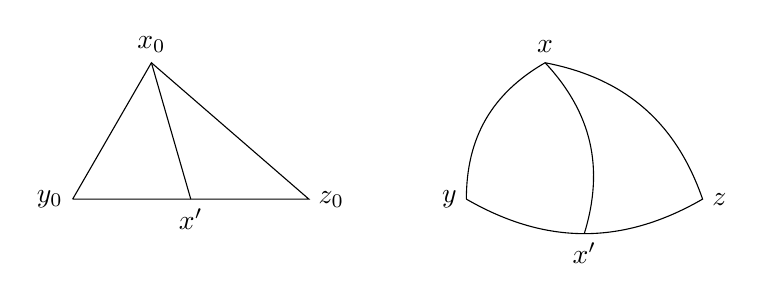
\begin{tikzpicture}
        \draw (5+0,0) node[left] {$y_0$} to (5+3,0) node[right] {$z_0$} to (5+1,1.732) node[above] {$x_0$} to (5+0,0);
        \draw (5+1,1.732) to (5+1.5,0) node[below] {$x'$};
        \draw (10+0,0) node[left] {$y$} to[bend right] (10+3,0) node[right] {$z$} to[bend right] (10+1,1.732) node[above] {$x$} to[bend right] (10+0,0);
        \draw (10+1,1.732) to[bend left] (10+1.5,-.43) node[below] {$x'$};
    \end{tikzpicture}
    \caption{Synthetic definition of Alexandrov curvature by triangles.}
\end{figure}
To define what it means (synthetically) to have a curvature bounded below by $K\in\RR$, not necessarily 0, we replace $\RR^2$ by these model spaces:
\begin{itemize}[nolistsep]
    \item the sphere $S^2(1/\sqrt{K})$ which has constant sectional curvature $K>0$;
    \item the plane $\RR^2$ which has constant sectional curvature $K=0$;
    \item the hyperbolic space $\HH^2(1/\sqrt{|K|})$ which has constant sectional curvature $K<0$.
\end{itemize}
\begin{defi}[Sectional curvature, analytic definition]
    \textit{[We do not give here the analytic definition of the sectional curvature. For the sake of having intuition on the conditions of \cref{prop:quad-cost-manifold-villani}, we give the (thus incomplete) definition of having an \emph{asymptotically nonnegative curvature}]}
    Let $M$ be a Riemannian manifold. We say that $M$ has \emph{asymptotically nonnegative curvature} if all sectional curvatures $\sigma_{x}$ at point $x$ satisfy $$\sigma_{x}\geq -\frac{C}{d(x_{0},x)^{2}}$$ for some positive constant $C$ and some $x_{0}\in M$.
\end{defi}
Toponogov's theorem makes the connection between both definitions. In particular, a complete simply connected Riemannian manifold has:
\begin{itemize}[nolistsep]
    \item (analytic) non-negative sectional curvature if and only if the function $f_{p}(x)=d(p,x)^2$ is 1-concave for all points $p$;
    \item (analytic) non-positive sectional curvature if and only if the function $f_{p}(x)=d(p,x)^2$ is 1-convex for all points $p$.
\end{itemize}



\section{Other notions}
    \subsection{Approximate differentiability}
    \begin{defi}[Approximate differentiability, \cite{villani2009optimal}]
        Let $U$ be an open set of a Riemannian manifold $M$, and let $f: U \to \mathbb{R} \cup\{\pm \infty\}$ be a measurable function. Then $f$ is said to be \emph{approximately differentiable} at $x \in U$ if there is a measurable function $\tilde{f}: U \to \mathbb{R}$, differentiable at $x$, such that the set $\{\tilde{f}=f\}$ has density 1 at $x$; in other words,
        $$\lim _{r \to 0} \frac{\operatorname{vol}\left[\left\{z \in B_r(x) ; f(z)=\tilde{f}(z)\right\}\right]}{\operatorname{vol}\left[B_r(x)\right]}=1\, .$$
        Then one defines the approximate gradient of $f$ at $x$ by the formula
        $$\tilde{\nabla} f(x)=\nabla \tilde{f}(x)\,.$$
        \label{def:approx-grad}
    \end{defi}

    \subsection{General definition of submodularity}
    \label{sec:submod-general}
    \begin{defi}
        Submodularity is more generally defined for functions defined on subsets of $\mathbb{R}^n$ of the form $\Zz=\Pi_{i=1}^n\Zz_{i}$ with each $\Zz_{i}$ a compact subset of $\mathbb{R}$ \cite{bach2019submodular}. A function $H:\Zz\to \mathbb{R}$ is then submodular if for all $z_{1},z_{2}$ in $\Zz$, $H(z_{1})+H(z_{2})\geq H(\max\{ z_{1},z_{2}\}  )+H(\min\{ z_{1},z_{2}\}  )$, where the min and max operations are applied component-wise.
        In our case where $c$ is a function over $\mathbb{R}\times\mathbb{R}$, not necessarily differentiable, this more general formulation of the submodularity becomes:
        \begin{equation*}
            \text{for all } x,y\in\mathbb{R},\text{ for all }\alpha,\beta\geq0,\quad c(x+\alpha,y)+c(x,y+\beta) \geq c(x,y)+c(x+\alpha,y+\beta)
        \end{equation*}
        and we recover the definition of \cref{sec:monotonicity}.
    \end{defi}


    \subsection{Numbered limb system}
        The notion of numbered limb system has been introduced in \cite{hestir1995supports} and applied to optimal transport by \cite{ahmad2011optimal,chiappori2010hedonic}.
        \begin{defi}[Numbered limb system]
            \label{def:nls}
            Let $X$ and $Y$ be Borel subsets of complete separable metric spaces. A relation $S \subset X \times Y$ is a \emph{numbered limb system} if there is a countable disjoint decomposition of $X=\cup_{i=0}^{\infty} I_{2 i+1}$ and of $Y=\cup_{i=0}^{\infty} I_{2 i}$ with a sequence of maps $f_{2 i}: \operatorname{Dom}(f_{2 i}) \subset Y \longrightarrow X$ and $f_{2 i+1}: \operatorname{Dom}(f_{2 i+1}) \subset X \longrightarrow Y$ such that $S=\cup_{i=1}^{\infty} \operatorname{Graph}(f_{2 i-1}) \cup \operatorname{Antigraph}(f_{2 i})$, with $\operatorname{Dom}(f_{k}) \cup \operatorname{Ran}(f_{k+1}) \subset I_{k}$ for each $k \geq 0$. The system has (at most) $N$ limbs if $\operatorname{Dom}(f_{k})=\varnothing$ for all $k>N$.
        \end{defi}
        \begin{figure}[!h]
            \centering
            \begin{tikzpicture}[
    scale=1.5,
]
    \begin{axis}[
        axis lines=left,
        domain=0:4,
        y domain=0:4,
        xticklabels={,,},
        yticklabels={,,},
        samples=50,
        y=1cm,
        x=1cm,
        ]
        \addplot[semithick,color=tabpurple,domain=0:1]{(2*(x-0.5))^2};
        \addplot[semithick,color=tabpurple,domain=1:2]{3.05+(2*(x-1.5)+1/3)^3-(2*(x-1.5)+1/3)^2-x};
        \addplot[semithick,color=tabpurple,domain=2:3]{3-(2*(x-2.5))^2};
        \addplot[semithick,color=white, domain=3:4]{x};
        \addplot[semithick,color=tabpurple,domain=0:1,y domain=0:1] ({1+(2*(x-0.5))^2},2+x);
        \addplot[semithick,color=tabpurple,domain=1:2,y domain=1:2] ({2.05+(2*(x-1.5)+1/3)^3-(2*(x-1.5)+1/3)^2-x},x);
    \end{axis}
        \draw (0.5,0) node[below] {$I_1$};
        \draw (1.5,0) node[below] {$I_3$};
        \draw (2.5,0) node[below] {$I_5$};
        \draw (3.5,0) node[below] {$\dots$};
        \draw (0,0.5) node[left] {$I_0$};
        \draw (0,1.5) node[left] {$I_2$};
        \draw (0,2.5) node[left] {$I_4$};
        \draw (0,3.5) node[left] {$\vdots$};
        \draw (3.5,3.5) node[tabpurple] {$\iddots$};
        % grid
        \draw[dashed,gray] (1,0) -- (1,3.8);
        \draw[dashed,gray] (2,0) -- (2,3.8);
        \draw[dashed,gray] (3,0) -- (3,3.8);
        \draw[dashed,gray] (0,1) -- (3.8,1);
        \draw[dashed,gray] (0,2) -- (3.8,2);
        \draw[dashed,gray] (0,3) -- (3.8,3);
\end{tikzpicture}
            \caption{Representation of a numbered limb system with $N$ limbs. The subsets $I_k$ are represented connected for visual convenience but do not need to be.}
            \label{fig:NLS2}
        \end{figure}
    \newpage
    \subsection{Lagrangian and Eulerian discretizations}

    \label{sec:types-disc}
        \begin{figure}[!h]
            \centering
            \begin{subfigure}[c]{.49\linewidth}
                \centering
                \includegraphics[width=.8\textwidth]{img/disc-lagrangian.png}
                \caption{Lagrangian formulation (point cloud). The discrete probability measure is $\sum_{i=1}^{n}\frac1n\delta_{x_{i}}$.}
            \end{subfigure}
            \hfill
            \begin{subfigure}[c]{.49\linewidth}
                \centering
                \includegraphics[width=.8\textwidth]{img/disc-eulerian.png}
                \caption{Eulerian formulation (histogram). The discrete probability measure is $\sum_{i=1}^{n}a_{i}\delta_{\hat x_{i}}$ with $a$ a probability vector and $(\hat x_{i})$ a regular grid on the domain.}
            \end{subfigure}
            \caption{Associating a discrete probability measure to a dataset $(x_i)_{i=1}^n$: Lagrangian and Eulerian methods. Image taken from \cite{vayer2020contribution}.}
            \label{fig:types-disc}
        \end{figure}

